\section{Experimental setup and control variables}
\label{sec:control_variables}

\begin{figure}[!ht]
 \centering
 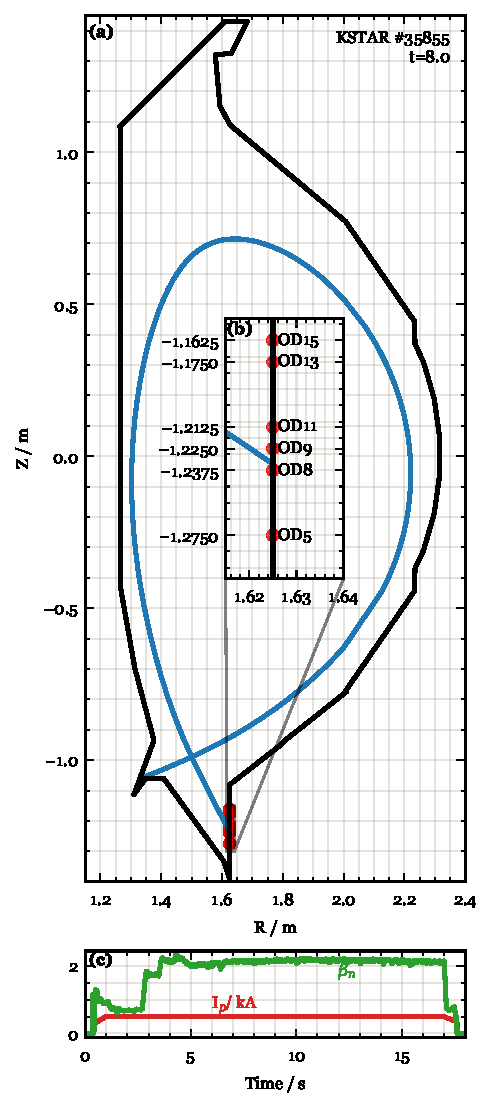
\includegraphics[width=\linewidth]{figures/RefShot.pdf}
 \caption{Reference shot \# 35855. (a) Showing last closed flux surface at t=8 seconds. The magnetic shape control was programmed to keep X point fixed which provided a sufficiently stable strike point on the realtime Langmuir Probe array. (b) Zoomed-in locations of realtime Outer Divertor (OD) Langmuir probes. (c) Plasma current (I$_p$) and $\beta_n$ for reference shot.}
 \label{fig:ref_shot}
\end{figure}

The experiment was conducted on standard single lower null H-mode plasma profile with reference shot KSTAR \# 35855 with the equilibrium profile as shown in Fig.\ref{fig:ref_shot}. The plasma shaping steps commensed by 7\~s and the shot was programmed for flat-top upto 17s providing 10s long window for detachment control experiment. For heat flux control, N$_2$ gas puffing was used. The heat flux control variable was tested with several different inputs.

First, we utilized previously develoed $A_{frac}$\cite{Eldon_2022_PPCF}, which is defined as the ratio of measured ion saturation current to modeled (using 2PM\cite{Leonard_2018_PPCF}) ion saturation current assuming fully attachment plasma. $A_{frac}$ is a convinient choice of control variable which is easily available in most tokamaks and allows for cross comparison among machines. If the strike point on the diverter tile is fixed in position well enough by the shape control system, a single close-by langmuir probe is enough to provide the ion saturation current required for $A_{frac}$ calculation. However,if the strike point control is not good enough, or if it is required to leave it as a free variable to allow for controlling other parameters in the shape control loop (as was the case in our experiments), then it is requried to estimate the true ion saturation current through measurements made by an Langmuir probe array. In our experiments, we chose the peak value from the langmuir probe array as the input to ion saturation current at strike point.

Langmuir probes would not be able to survive high heat flux in burning plasma future reactors. In general, such reactors would be severely limited in the number of realtime sensors available for control systems because of high neutron fluence and heat flux in vacuum vessel, and thus alternate control variables need to be searched for. Towards this goal, we tested a prototype of a machine-learning-based surrogate model of 2D UEDGE, DivControlNN. The employed version of DivControlNN is trained on $\approx$ 70,000 2D UEDGE simulations of KSTAR. The diffusion coefficient profile is assumed for a typical H-mode shot which can be scaled as an input to the model. The training dataset scanned core electron density ($1.08 \times 10^{19} - 6.62 \times 10^{19}$ m$^{-3}$), plasma current ($600-800$ kA), injected total power through NBI and ECH ($1-8$ MW), impurity fraction with respect to Deuterium density ($0-0.04$), and scaling of diffusion coefficient profile with a factor ($0.6 - 2$). This provided a widely applicable surrogate model which gives steady state values of heat flux, ion saturation current, and electorn temperature along the two divertors, electron density and temperature at upstream point of midplane, and total radiated power, power fraction radiated from divertor, and peak radiation power location in the poloidal cross-section of the device. The model generates output within 10\% error from the 2D UEDGE outpout.

This preliminary model, however, has been trained on 2D UEDGE simulations of KSTAR with carbon divertor and carbon as the sole impurity species. So it does not reflect the same Tungsten divertor system in which it was tested. There were several other limitations to the realtime input provided to the model. At KSTAR, the total input power from NBI and ECH sources is not completely available in realtime PCS and we had to input a feedforward signal matching the programmed rate of some sources that got summed with the other sources whose power was avaialble in realtime. Similarly, there was no reliable input for impurity fraction in plasma and we created an adhoc gas accumulation model which measured impurity fraction by taking ratio of total puffed impurity with total puffed Deuterium gas with estimated decay rates to model the effect of pumping and wall adsorption. Finally, the diffusion coefficient scaling factor was set to 1.0 for loack of any better realtime information on it. We are in the process of training a model in Tungsten divertor environment and with gas flow rate as an input by running the simulations with multi-charge-state impurity model. This, along with improvements in realtime data availability in KSTAR would empower the model to provide outputs with higher confidence in future.
